\documentclass[letterpaper, 11pt]{report}
\usepackage{setspace}
\usepackage[
    backend=biber,
    style=numeric,
]{biblatex}
\usepackage{graphicx}
\usepackage{amsmath}
\usepackage{amssymb}
\usepackage{hyperref}
\usepackage{titlesec}
\usepackage{geometry}
\usepackage{tocloft}
\usepackage{tabularx}
\usepackage{lipsum}
\usepackage{xcolor}

\addbibresource{references.bib}
\geometry{
    left=1in,
    right=1in,
    top=1in,
    bottom=1in,
}

\title{\LARGE 2024 Citadel Datathon Report\\[0.5\baselineskip]
\large Breaking the Cycle: The True Cost of Processed Food in the United States}
\author{\large Angela Busheska, Sheldon Lewis, Matthew Liu, Adel Müürsepp}
\date{\normalsize August 4 2024}
    
\renewcommand\thesection{\arabic{section}}

% Redefine section format for main sections of the document
\titleformat{\section}
  {\normalfont\Large\bfseries}{\thesection}{1em}{}

% No extra space before or after sections
\titlespacing*{\section}{0pt}{1.5\baselineskip}{0.5\baselineskip}

\renewcommand{\cfttoctitlefont}{\LARGE\bfseries}
\renewcommand{\cftaftertoctitle}{\hfill} % Adjusts spacing after title
\renewcommand{\cftsecnumwidth}{2em}
\renewcommand{\cftsubsecnumwidth}{3em}
\renewcommand{\cftsubsubsecnumwidth}{4em}
\renewcommand{\cftsecindent}{0em}
\renewcommand{\cftsubsecindent}{2em}
\renewcommand{\cftsubsubsecindent}{5em}
\renewcommand{\cftsecfont}{\color{blue}\bfseries}
\renewcommand{\cftsubsecfont}{\color{blue}}
\renewcommand{\cftsubsubsecfont}{\color{blue}}
\renewcommand{\cftsecpagefont}{\bfseries}
\renewcommand{\cftsubsecpagefont}{}
\renewcommand{\cftsubsubsecpagefont}{}

\newcommand{\tocsection}[1]{\addcontentsline{toc}{section}{\color{blue}#1}}
\newcommand{\tocsubsection}[1]{\addcontentsline{toc}{subsection}{\color{blue}#1}}
\newcommand{\tocsubsubsection}[1]{\addcontentsline{toc}{subsubsection}{\color{blue}#1}}

\begin{document}

\maketitle

\pagenumbering{roman}

\renewcommand{\contentsname}{Table of Contents}
\tableofcontents

\newpage
\onehalfspacing
\setcounter{page}{1}
\pagenumbering{arabic}

\section{Executive Summary}

% To be written after the findings are done

Processed foods have become integral to the American diet, driven by their convenience and low cost. However, the proliferation of fast food and other ultra-processed foods has profound implications for public health and socioeconomic stability. This report delves into the cycle perpetuated by the financial interests of corporations that produce and market processed foods. Our analysis reveals a cycle where corporate profitability comes at the expense of public health and economic well-being. Key findings highlight how the strategic interests of these corporations contribute to a cycle of poor mental health, low income, adverse employment conditions, and deteriorating physical health. Through comprehensive statistical analyses, we demonstrate the significant impacts of processed food prevalence on various socioeconomic and health indicators. The report underscores the need for targeted policy interventions to break this cycle and promote a healthier, more equitable society.

\section{Introduction}

\subsection{Background}

% Processed foods, including fast food, have become a staple in American diets, providing convenience at the cost of health. Despite widespread awareness of the negative health impacts, consumption remains high, driven by economic factors and corporate marketing strategies. This report examines the broader implications of this dietary trend, focusing on mental health and economic outcomes.

The surge of ultra-processed foods (UPFs) and fast food chains in the United States has deepened existing health and socioeconomic disparities. UPFs, stripped of nutrients and packed with additives, are widely consumed due to their convenience and low cost, especially in areas known as food deserts—regions where access to healthy, affordable food is limited. In these neighborhoods, often home to low-income and minority populations, fast food and convenience stores dominate, leaving residents with little choice but to rely on unhealthy options.

Aggressive marketing by food corporations targets the most vulnerable—children, minorities, and low-income communities—further entrenching unhealthy eating habits. This relentless promotion perpetuates a cycle of poor health, where reliance on cheap, unhealthy food leads to rising rates of obesity, diabetes, and heart disease. The introduction of fast food into struggling communities often becomes a default choice, reinforcing this cycle and exacerbating economic and health challenges.

Breaking free from this cycle requires more than individual education—it demands systemic change. We must reimagine food environments by investing in local food systems that offer fresh, affordable options and enacting policies that limit fast food proliferation in vulnerable areas. Only by addressing these structural issues can we hope to reverse the epidemic of diet-related diseases and promote health equity.

The rise of UPFs and fast food is not just a matter of convenience—it's a public health crisis that traps communities in cycles of poor health and economic disadvantage. To build a healthier future, we must dismantle this cycle and create a food environment that supports well-being for all. The report examines the mental health, self-reported physical health and economic benefits in communities and aims to propose solutions for the future.



\subsection{Objective and Research Questions}

The objective of this study is to investigate the multifaceted impacts of ultra-processed foods (UPFs) and fast food prevalence on various aspects of public health and socioeconomic conditions in the United States. By examining the relationship between fast food introduction and its effects on mental health, self-reported physical health, and economic outcomes across different demographic and socioeconomic contexts, this study aims to uncover the broader impact on communities of the introduction to more fast food options.

The key research questions guiding this study are:

\begin{itemize}
    \item How does the prevalence of fast food establishments affect different response variables, including mental health outcomes, economic conditions, and self-reported physical health metrics, particularly in communities with varying levels of income, racial composition, and rurality?
    \item How do these impacts differ across socioeconomic and demographic clusters, and what patterns emerge that can inform targeted public health interventions?
    \item How can the findings of this study inform targeted public health interventions aimed at mitigating the negative impacts of fast food on vulnerable populations and could healthy fast food be an option?
\end{itemize}




\subsection{Variables of Interest}
To address these questions, we examine a range of variables, including:
\begin{itemize}
    \item \textbf{Health Outcomes:} Average Number of Mentally Unhealthy Days, obesity rates, diabetes prevalence, heart disease rates.
    \item \textbf{Economic Indicators:} Household income, unemployment rates, employment conditions in the fast food industry.
    \item \textbf{Dietary Habits:} Consumption rates of soda, fast food, and other ultra-processed foods.
    \item \textbf{Corporate Metrics:} Stock prices, profit margins, and ESG (Environmental, Social, and Governance) scores of major fast food corporations.
\end{itemize}

\subsection{Methodology}

Our analysis employs a comprehensive methodology, including data loading and preprocessing, exploratory data analysis (EDA), clustering, propensity score matching, and mixed linear model regression. We focus on the period from 2014 to 2022, using county-level data to ensure detailed and localized insights. Key techniques include:
\begin{itemize}
    \item \textbf{KMeans Clustering:} To group counties with similar socioeconomic and demographic characteristics.
    \item \textbf{Propensity Score Matching:} To control for confounding variables and create balanced comparison groups.
\end{itemize}

% Actually here needed how UPF is part of American culture and diet a little bit
% The hidden costs of these dietary choices are staggering in a nation where the convenience of processed foods has become a staple of daily life. Despite the ubiquitous presence of fast food and processed snacks, their impact on quality of life and the economy often goes unnoticed. Heart disease, the leading cause of death in the United States, claims over 697,000 lives annually, while the diabetic population has skyrocketed to over 37 million Americans. Every year, \$327 billion dollars is spent on diabetes care alone.
% %https://www.cdc.gov/brfss/


% So why do we keep eating fast food? The link between processed food and illness is analytically obvious, but what's not is the underlying cycle of consumption, employment, poverty, convenience, and corporate greed that traps both workers and consumers in vicious cycles of over-consumption for the benefit of the ultra-rich.


% % https://www.medrxiv.org/content/10.1101/2024.02.16.24302894v1.full
% Ultra-processed foods differ from other processed foods like cheese or pasta in the way that they have been treated with chemicals to have a longer shelf life and taste better. However, this comes with the downside of losing the nutritional benefits. In addition, a study has found that eating UPF as compared to not processed foods makes people eat, on average, 500 calories more per day. 

% % Thoughts: discuss habits and culture maybe in relation to demographic and cultural info

% Fast food consumption didn’t necessarily fall during the COVID-19 pandemic; it simply became delivery-based instead of traditional in-person dining. Stocks of major fast-food chains experienced a brief plummet during March and April 2024 but have since rebounded as delivery services became more prominent. Despite this shift, the number of employees in these sectors remained significant, highlighting the persistent demand for fast food.


% The main categories that the impact of UPF has on the American population were divided into health-related, mental health and life satisfaction-related, and finally, economic benefit/cost. It is well known that the "fast food cycle" traps some demographic groups and regions more gravely, i.e., the existence of food deserts. Therefore, we stipulate that the demographic composition of the environments plays a role in how the availability and marketing of processed foods affects the livelihood of American people across the country. 

% Here maybe also mention that we wished to analyze the type of jobs that had the most growth if some stocks rose

% And then we also characterized fast food restaurants landscape and analyzed stocks

% Discuss that maybe fast food is the main convenient option for some counties. So we investigate if fast food corporations are pushing the demand and making low income families dependent on fast food if they get introduced to the county




\section{Exploratory Data Analysis}

Given the provided datathon datasets, we wanted to further understand the correlation between obesity, meat production, and stock sales. In this report, we look at the following three comparisons: Meat Production vs Unemployment Rate, Sugar Prices and Consumption Over Time and Comparison between meat production and stock prices.


\subsection*{Potential Predictive Variables}

First, the effect of the introduction of processed foods to a county was investigated on physical and mental health outcomes. Note that this is a county-level analysis.

\begin{table}[h]
\centering
\caption{Features for Linear Regression}
\begin{tabularx}{\textwidth}{|p{0.25\textwidth}|X|}
\hline
\textbf{Category} & \textbf{Variables}                                        \\ \hline
Introduction of UPFs & \vspace{-0.3cm} \begin{itemize}
    \item \% change of fast-food restaurants/1,000 people (2011-16) \cite{foodenvatlas}
    \item \% change of convenience stores/1,000 people  (2011-16) \cite{foodenvatlas}
\end{itemize} \\ \hline
Environmental Factors & \vspace{-0.3cm} 
\begin{itemize}
    \item \% of rural population \cite{countyhealthrankings}
    \item \% change in proportion of rural population  (2011-2016) \cite{countyhealthrankings}
    \item \% of population with low access to grocery stores (2010) \cite{foodenvatlas}
    \item Indicator for persistent poverty county (2010) \cite{foodenvatlas}
    \item Indicator for metro/nonmetro county (2010) \cite{foodenvatlas}
    \item Indicator for population-loss county (2010) \cite{foodenvatlas}
    \item Average household income (2011) \cite{countyhealthrankings}
    \item Recreation/fitness facilities per 1,000 people (2011) \cite{foodenvatlas}
    \item Grocery stores per 1,000 people (2011) \cite{foodenvatlas}
\end{itemize} \\ \hline
Demographic Factors & \vspace{-0.3cm} \begin{itemize}
    \item \% of African American population (2011) \cite{countyhealthrankings}
    \item \% of Asian population (2011) \cite{countyhealthrankings}
    \item \% of Hispanic population (2011) \cite{countyhealthrankings}
    \item \% of obese adults (2011) \cite{countyhealthrankings}
    \item Number of primary care physicians per 1,000 people (2011) \cite{countyhealthrankings}
\end{itemize}\\ \hline
Food Assistance Program & \vspace{-0.3cm} \begin{itemize}
    \item SNAP-authorized stores per 1,000 people in 2012 \cite{foodenvatlas}
    \item SNAP benefits per capita (\$) in 2012 \cite{foodenvatlas}
    \item WIC redemptions per capita (\$) in 2011 \cite{foodenvatlas}
\end{itemize} \\ \hline
\end{tabularx}
\label{table:feature_variables}
\end{table}

\begin{table}[h]
\centering
\caption{Potential Considered Response Variables}
\begin{tabularx}{\textwidth}{|p{0.25\textwidth}|X|}
\hline

\textbf{Category} & \textbf{Variables}                     \\ \hline
Health Outcomes (2011-16, data from County Health Rankings 
\cite{countyhealthrankings}) & \vspace{-0.3cm} \begin{itemize}
    \item \% change in diabetes among adults
    \item \% change in obesity among adults
    \item \% change in binge drinking among adults
    \item \% change in physical inactivity
    \item \% change in mentally unhealthy days
    \item \% change of people in fair/poor health
\end{itemize} \\ \hline
\end{tabularx}
\label{table:response_variables}
\end{table}
Note that the demographic population data was available for year 2010 in Food Environment Atlas but instead, for the data to be more accurate, County Health Rankings was used.

Secondly, the economic benefits of the introduction of processed food establishments to a county were investigated. 


% \begin{table}[h]
% \centering
% \caption{Predictor and Response Variables for Multivariate Regression}

% \begin{tabularx}{\textwidth}{|l|X|}
% \hline
% \textbf{Category}                  & \textbf{Variables}                                        \\ \hline
% \multicolumn{2}{|c|}{\textbf{Predictor Variables}}                                             \\ \hline
% Introduction of Processed Foods    & - Percent change of fast-food restaurants/ 1000 pop between years 2011-2016 per county\newline
%                                    - Percent change of convenience stories/ 1000 pop between years 2011-2016 per county   \\ \hline
% Environmental Factors              & - Metro/nonmetro counties, 2010 \newline
%                                     - \% Rural, 2011 \newline
%                                     - Percent change in proportion rural population, 2011 - 2016 \newline
%                                     - Persistent-poverty counties, 2010 \newline
%                                     - Population-loss counties, 2010 \\ \hline
% Demographic Factors                & - Percent of population African American, 2011 \newline
%                                    - Percent of population Asian, 2011 \\ \hline

% \multicolumn{2}{|c|}{\textbf{Response Variables}}                                              \\ \hline
% Economic Benefits         & - Percent change in median household income, 2011-2016 Household (County Health Rankings 2011 Additional Measure Data Household Income 2011, 2016. Calculate)\newline
%                                     - Percent change in unemployment, 2011-2016 (County Health Rankings 2011 Ranked Measure Data % unemployed 2011, % Unemployed 2016. Calculated) 
%                                     \\ \hline

% \end{tabularx}
% \label{table:predictor_response_variables}
% \end{table}

% Here put different symbols for data years 2010, 2011, 2012 and for different data sources and explain why they are good for approximations


\subsection{Meat Production and Unemployment Rate}

\begin{table}[h!]
\centering
\begin{tabular}{|c|c|c|}
\hline
          & Production & Estimate  \\ \hline
Production & 1.000000   & 0.450953  \\ \hline
Estimate   & 0.450953   & 1.000000  \\ \hline
\end{tabular}
\caption{Production and Estimate Correlation Matrix for Meat Production vs Unemployment Rate}
\label{table:correlation}
\end{table}

\begin{figure}[h!]
    \centering
    \includegraphics[width=\linewidth]{images/image5.png}
    \caption{Regression Analysis of Meat Production vs. Unemployment Rate }
    \label{fig:employees}
\end{figure}

The moderate $R^2$ value (0.203) suggests that meat production explains about 20.3 percent of the variance in unemployment rates. The positive coefficient indicates that an increase in meat production is associated with an increase in the unemployment rate, though this relationship is not particularly strong.

\begin{table}[h!]
\centering
\begin{tabular}{|l|r|}
\hline
Parameter                           & Value        \\ \hline
Intercept                           & -417,463.01  \\ \hline
Coefficient                         & 6,785.21     \\ \hline
R\textsuperscript{2} (Coefficient of Determination) & 0.203        \\ \hline
\end{tabular}
\caption{Regression Analysis Results for Meat Production vs. Unemployment Rate}
\label{table:regression}
\end{table}


\subsection{Sugar Prices and Consumption}

As sugar prices decrease, consumption also tends to decrease, though not as steeply. This might suggest that factors other than price are influencing sugar consumption trends.

\begin{figure}[h!]
    \centering
    \includegraphics[width=\linewidth]{images/image1.jpg}
    \caption{Average Sugar Prices and Consumption Over Time }
    \label{fig:employees}
\end{figure}


\subsection{Meat Production and Stock Prices}

For this segment, we are merging the data sets of meat production over time with the average stock price for a given year. Following the analysis, one can see that the stock price is growing while having a steady meat production over the years.

\begin{figure}[h!]
    \centering
    \includegraphics[width=\linewidth]{images/image6.jpg}
    \caption{Average Sugar Prices and Consumption Over Time }
    \label{fig:employees}
\end{figure}


\subsection*{Facts by state}
\begin{itemize}
    \item \textbf{PR (Puerto Rico)}: Has the highest positive correlation (0.1376), indicating a strong positive relationship.
    \item \textbf{VI (Virgin Islands)}: Has the highest negative correlation (-0.1641), indicating a strong negative relationship.
    \item \textbf{MA (Massachusetts)}: Also shows a significant positive correlation (0.1131), suggesting a notable positive relationship.
    \item \textbf{ID (Idaho)}: Displays a relatively high positive correlation (0.0704).
    \item \textbf{NH (New Hampshire)}: Shows a high positive correlation (0.0891).
\end{itemize}

The analysis reveals complex interrelationships among food production, economic indicators, and consumer behavior. Notably, the data indicate an inverse relationship between sugar prices and consumption, suggesting that factors beyond cost significantly influence consumer choices. This trend may reflect an increasing consumer awareness of health implications and a growing preference for nutritionally superior options, which could be leveraged to promote healthier fast food alternatives.
The observed pattern of steady meat production coupled with rising stock prices in the food industry suggests that economic growth in this sector is not exclusively dependent on traditional meat products. This diversification in revenue sources warrants further investigation.
Based on these preliminary findings, we formulated two primary research questions:

What is the economic and environmental footprint of the emerging "healthy fast food" sector (exemplified by brands such as Chipotle Mexican Grill and Cava Group) in comparison to traditional fast food establishments? This investigation aims to quantify differences in economic impact, employment patterns, nutritional profiles, and environmental sustainability between these two categories of food service providers.
Given that sugar consumption appears to be decoupled from price fluctuations, what are the potential associations between dietary habits (particularly sugar and soda consumption) and mental health outcomes across various geographic and demographic segments?

These research questions are designed to provide a comprehensive understanding of the evolving fast-food landscape and its multifaceted impacts on public health, the economy, and the environment.


\subsection*{Relation of Demographic and Environmental Factors on Economic Impact Upon Introduction of Fast Food}

\begin{figure}[h!]
    \centering
    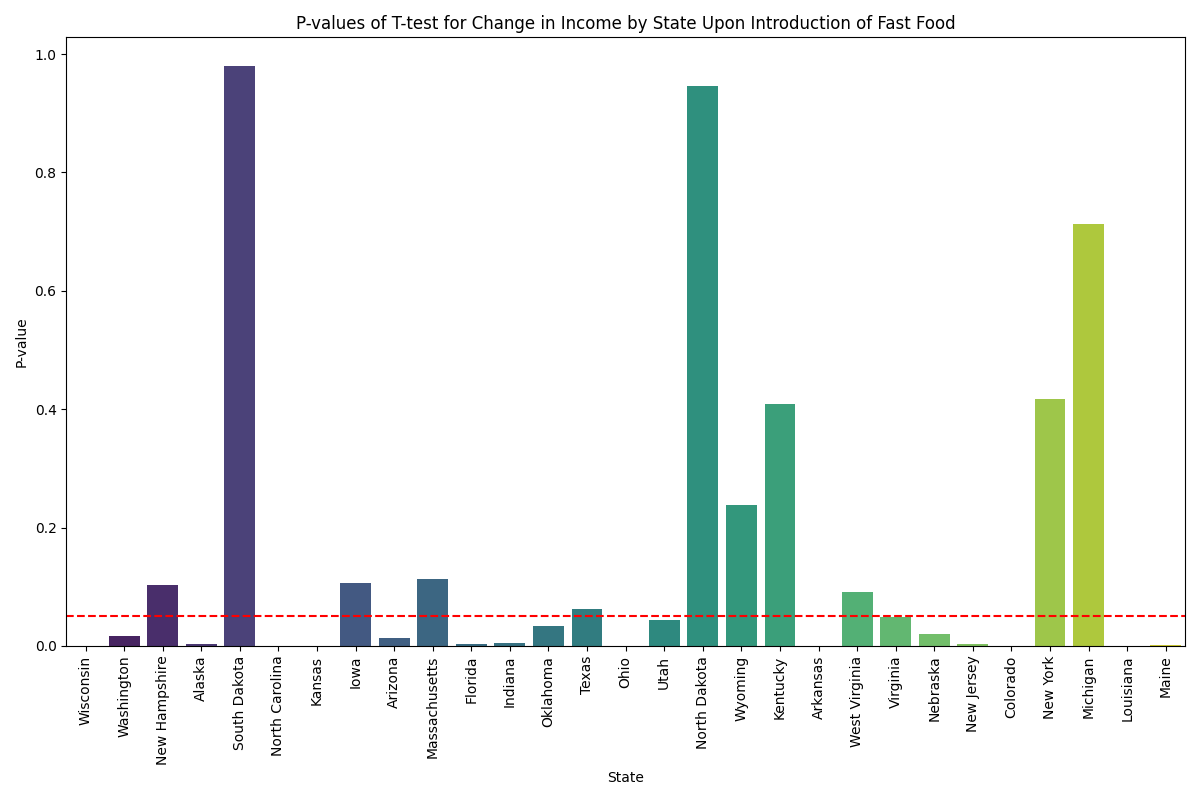
\includegraphics[width=\linewidth]{propensity matching introduction of fast food income}
    \caption{Effect on Income By State Upon Introduction of Fast Food}
    \label{fig:employees}
\end{figure}

It was found that on the national level the introduction of fast food did not have a large effect. However, different regions on the state and county level had significant increases or decreases in income, physical or mentalh health metrics. This prompted a further investigation into how different regions are affected by introduction of fast food.
\newpage
\section{Discovery}

\subsection{Investigating the Impact of Fast Food Prevalence on Mental Health Outcomes}

\subsubsection{Clustering and Data Overview}
This analysis leverages clustering techniques to group counties based on a combination of socioeconomic and demographic characteristics, which are critical in understanding how changes in fast food prevalence may affect public health, specifically mental health outcomes. The clustering features used in the analysis include:

\begin{itemize}
    \item Rural population percentage in 2011 (\texttt{Rural\_2011})
    \item Household income in 2011 (\texttt{Household Income\_2011})
    \item Percentage of African American residents in 2011 (\texttt{African American\_2011})
    \item Percentage of Asian residents in 2011 (\texttt{Asian\_2011})
    \item Percentage of Hispanic residents in 2011 (\texttt{Hispanic\_2011})
    \item Obesity rate in 2011 (\texttt{Obese\_2011})
\end{itemize}


These features were selected to capture the diversity in rurality, income, racial composition, and pre-existing health conditions across counties. The dataset encompassed 2901 counties, even though there are 3143 counties in the United States. This means some counties had missing data for one of the years studied. The study focused on the years 2012-2017, chosen due to the availability of comprehensive data on fast food restaurants, which limits the temporal scope of the analysis but ensures robustness in the findings. The pairwise relationships between features are shown in the appendix.

\subsubsection{Study Overview}
The analysis was designed to explore the nuanced impacts of fast food restaurant prevalence on mental health across counties with varying socioeconomic and demographic profiles. Recognizing that the relationship between fast food availability and health outcomes is multifaceted and context-dependent, the study employed several key steps:

\paragraph{Data Loading and Preprocessing:}
The dataset was meticulously prepared by first dropping rows with missing values in critical features, ensuring that the subsequent analysis would be based on complete and reliable data. A binary treatment variable was then constructed to identify counties that experienced a significant increase in fast-food restaurants. This binary distinction allows for a clear comparison between treated and control groups in the later stages of the analysis.

\paragraph{Clustering:}
KMeans clustering was applied to group counties into distinct clusters based on their socioeconomic and demographic characteristics. This step was crucial for two main reasons: First, it allowed the analysis to account for the inherent heterogeneity among counties, ensuring that comparisons were made within more homogeneous groups. Second, it facilitated the investigation of whether the impact of fast food prevalence varied according to the socioeconomic and demographic context of the counties.

\paragraph{Propensity Score Matching (PSM):}
Given the observational nature of the data, PSM was employed to reduce selection bias and approximate a randomized controlled trial. For each cluster, a logistic regression model was used to calculate propensity scores, which estimate the probability that a county would receive the treatment (i.e., a significant increase in fast-food restaurants). Nearest Neighbors Matching was then applied to match treated counties with control counties that had similar propensity scores, thereby creating a balanced comparison group for the t-test.

\paragraph{t-test:}
A t-test was conducted within each cluster to statistically compare the change in mental health outcomes, particularly mentally unhealthy days, between treated and control counties. This test helps determine whether the observed differences in mental health outcomes are statistically significant and can be attributed to the changes in fast-food restaurant prevalence.

\paragraph{Visualization:}
To enhance interpretability, the p-values of the t-tests across clusters were visualized. This step is critical in identifying which clusters exhibited statistically significant effects, thereby highlighting areas of potential concern for public health interventions.

\subsubsection{Techniques and Their Purpose}
The main three statistical techniques utilized were clustering, propensity score matching (PSM) and t-tests.

\noindent \textbf{Clustering (K-means)}: 

\begin{itemize}
    \item \textbf{Purpose:} The primary purpose of clustering was to group counties with similar characteristics—such as rurality, income, and racial composition—thereby ensuring that the analysis compares like with like. By segmenting counties into clusters, the analysis could better capture the contextual nuances that influence how fast food availability impacts mental health.

    \item \textbf{Statistical Benefit:} Clustering minimizes confounding effects that could arise if dissimilar counties were compared directly. This approach allows for more accurate inferences regarding the impact of fast food prevalence within specific socioeconomic and demographic contexts.
\end{itemize}

\noindent \textbf{Propensity Score Matching (PSM):}

\begin{itemize}
\item \textbf{Purpose:} PSM was employed to create a quasi-experimental design by matching treated counties with control counties that had similar propensity scores. This method helps ensure that the differences in mental health outcomes between treated and control groups can be more confidently attributed to the treatment rather than to pre-existing differences.

\item \textbf{Statistical Benefit:} PSM controls for confounding variables that could bias the estimated treatment effect, thereby enhancing the credibility of the causal inferences drawn from the analysis. By mimicking a randomized controlled trial, PSM allows for a more rigorous assessment of the impact of fast food prevalence.

\end{itemize}

\noindent \textbf{t-test:}
\begin{itemize}
    \item \textbf{Purpose:} The t-test was used to statistically compare the mean change in mental health outcomes between treated and control counties within each cluster. This test provides a formal mechanism for assessing whether the observed differences are statistically significant.
    \item \textbf{Statistical Benefit:} The t-test quantifies the likelihood that the differences in mental health outcomes are due to chance, offering a clear indicator of whether the treatment (increased fast food prevalence) had a measurable impact on mental health within each cluster.

\end{itemize}

\subsubsection{Cluster-Specific Insights and Policy Implications}
\paragraph{Cluster-Specific Insights:}
The clustering and subsequent analysis revealed that the impact of fast food prevalence on mental health is not uniform across all counties. Instead, the effects are highly context-dependent, varying significantly based on the socioeconomic and demographic characteristics of each cluster. For instance, clusters with high p-values indicated that there was no significant difference between treated and control groups, suggesting that in these clusters, the increase in fast food prevalence did not have a noticeable impact on mental health. Conversely, clusters with low p-values exhibited significant effects, indicating a strong association between fast food prevalence and mental health outcomes in these areas.

\paragraph{Policy Implications:}
The findings underscore the importance of targeted public health interventions. In clusters characterized by low income and high obesity rates, more stringent regulations on fast food establishments may be necessary to mitigate the adverse effects on mental health. Additionally, the analysis suggests that interventions should be tailored to the specific needs and vulnerabilities of each cluster, rather than adopting a one-size-fits-all approach. For example, counties with significant minority populations and low-income levels might benefit from policies that not only regulate fast food availability but also enhance access to healthier food options and healthcare services.

\paragraph{Future Research Directions:}
This analysis opens several avenues for future research. One potential direction is to explore the mechanisms through which fast food availability affects mental health, focusing on mediating factors such as dietary changes, physical activity, and stress levels. Additionally, future studies could examine the long-term effects of fast food prevalence on mental health and other health outcomes, considering how these impacts evolve over time in different socioeconomic contexts.

\paragraph{Causal Inference:}
The combination of PSM and clustering in this study provides a strong framework for causal inference, albeit with some limitations. While this approach cannot fully replicate the conditions of a randomized controlled trial, it offers a robust method for estimating the causal effect of fast food prevalence on mental health. The findings from this analysis, therefore, should be interpreted with an understanding of the underlying assumptions and potential sources of bias.

\subsubsection{Cluster Summaries and Qualitative Analysis}

\noindent The figure below illustrates the p-values of the T-test conducted to assess the change in mental health outcomes across different clusters following the introduction of fast food establishments. The red dashed line represents the significance threshold of p = 0.05, helping to identify which clusters exhibit statistically significant changes in mental health due to fast food prevalence.

% The figure environment for the image and its caption
\begin{figure}[h!]
    \centering
    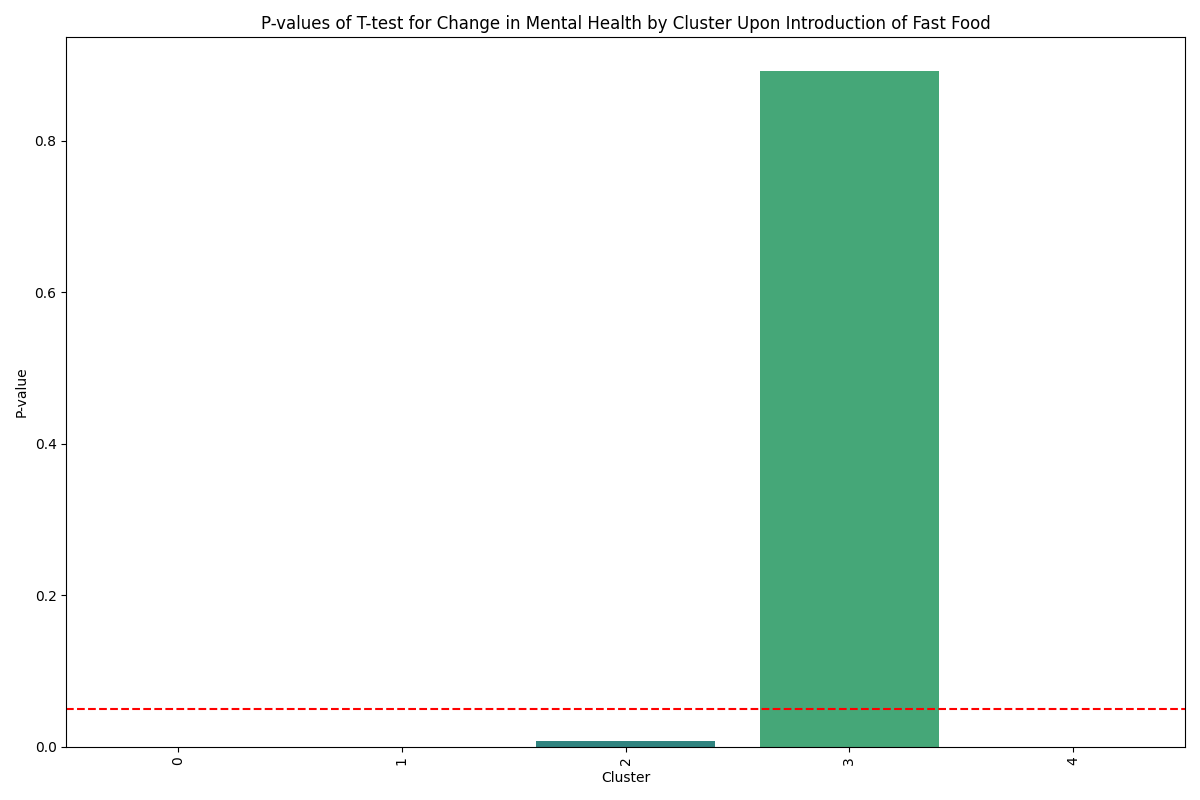
\includegraphics[scale=0.4]{propensity_matching_clusters_mental_health.png}
    \caption{P-values of T-test for Change in Mental Health by Cluster Upon Introduction of Fast Food}
    \label{fig:mental_health_pvalues}
\end{figure}





The following summaries provide detailed insights into the characteristics and health outcomes of each cluster:

\paragraph{Cluster 0:} 
This cluster comprises moderately rural counties with middle-income levels and moderate racial diversity. Obesity rates are typical of the national average, reflecting a balance between rural and urban influences. The analysis suggests that in these counties, changes in fast food availability have a substantial impact on obesity and, by extension, mental health outcomes. The strong positive t-statistic observed in this cluster underscores the sensitivity of these counties to changes in their food environment, making them a key target for public health interventions. 


\paragraph{Cluster 1:} 
Cluster 1 is characterized by highly rural, economically disadvantaged counties with a high percentage of African American residents and elevated obesity rates. The analysis reveals a complex relationship between fast food availability and health outcomes in these counties. Interestingly, the negative t-statistic suggests that an increase in fast food availability may be associated with a decrease in obesity rates in this cluster. This counterintuitive finding could be indicative of underlying socioeconomic factors that influence dietary behaviors differently in these communities. For example, increased fast food availability might correlate with other changes, such as increased economic activity or shifts in food consumption patterns that are not immediately harmful.

\paragraph{Cluster 2:} 
This cluster includes very rural counties with low to moderate incomes and low racial diversity. Obesity rates in these counties are moderate, and the analysis indicates that changes in fast food availability have a measurable impact on health outcomes. The moderately positive t-statistic suggests that while these counties are affected by changes in fast food prevalence, the impact is less pronounced than in more vulnerable clusters. This finding may reflect the relative isolation of these counties, where changes in the local food environment can have significant but not overwhelming effects on public health.

\paragraph{Cluster 3:} 
Cluster 3 represents urbanized, affluent counties with significant ethnic diversity and lower obesity rates. The analysis shows that in these counties, changes in fast food availability have little to no measurable impact on mental health outcomes. The near-zero t-statistic suggests that these communities have robust protective factors—such as better access to healthcare, healthier food options, and higher health literacy—that buffer against the potential negative effects of fast food proliferation. This resilience highlights the importance of socioeconomic status and access to resources in moderating the health impacts of the food environment.

\paragraph{Cluster 4:} 
Counties in Cluster 4 are characterized by low rural populations, higher income levels, and moderate racial diversity. The relatively low obesity rate in this cluster suggests that residents have good access to healthcare and healthier lifestyle options. However, the strong positive t-statistic observed in this cluster indicates that even in affluent areas, changes in fast food availability can have a significant impact on health outcomes. This finding underscores the importance of considering the cumulative effects of fast food availability, even in communities that might otherwise appear resilient.

\subsubsection{Qualitative Conclusions Based on P-Values and Cluster Composition}

For each of the clusters, the plot about the "Treated" and "Control" groups was analyzed. For example, in the plot for Cluster 0, the "Treated" group shows a higher median change in poor health, indicating a negative health impact from increased fast food presence. The positive t-value (3.39) and low p-value (0.001) suggest this difference is statistically significant. Similar analyses were applied to other clusters.

% The figure environment for the image and its caption
\begin{figure}[h!]
    \centering
    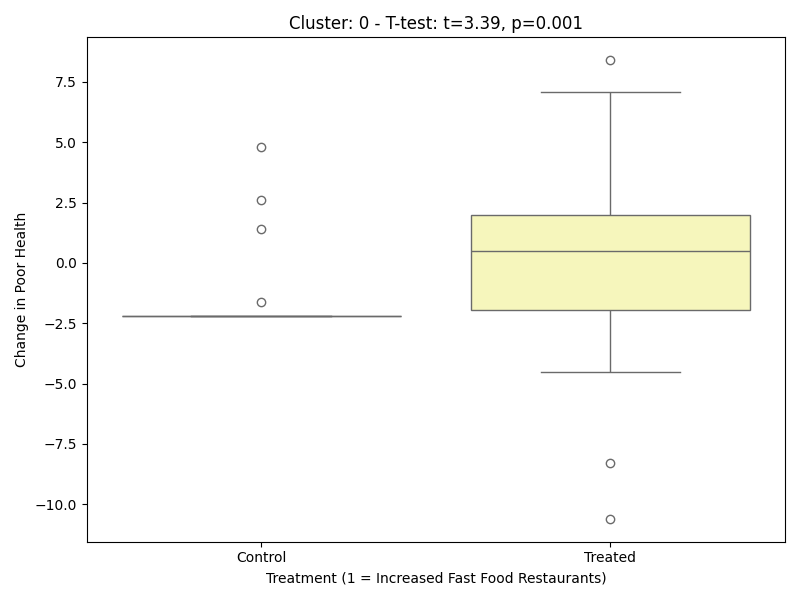
\includegraphics[scale=0.4]{cluster_0_fast_food_mental_health.png}
    \caption{P-values of T-test for Change in Mental Health by Cluster Upon Introduction of Fast Food}
    \label{fig:mental_health_pvalues}
\end{figure}

The qualitative analysis of the p-values and t-statistics across clusters offers several key insights:

\begin{itemize}
    \item \textbf{Cluster 0:} The strong positive t-statistic suggests that changes in fast food availability have a substantial impact on outcomes like obesity, making these counties a critical focus for public health interventions.
    \item \textbf{Cluster 1:} The negative t-statistic indicates a complex and potentially counter-intuitive relationship between fast food availability and obesity, highlighting the need for further research to understand the underlying dynamics in these economically disadvantaged, rural counties.
    \item \textbf{Cluster 2:} The moderately positive t-statistic suggests that while these very rural counties are affected by changes in fast food prevalence, the impact is more moderate, possibly due to the counties' relative isolation and other mediating factors.
    \item \textbf{Cluster 3:} The near-zero t-statistic reflects the resilience of affluent, urbanized counties to changes in fast food availability, likely due to strong protective factors such as access to diverse food options and healthcare.
    \item \textbf{Cluster 4:} The strong positive t-statistic in this cluster indicates that even in affluent areas, fast food availability can significantly influence health outcomes, suggesting that no community is entirely immune to the broader public health implications of an increasingly processed food environment.
\end{itemize}

\paragraph{Conclusion: Inequality, Rurality, and Racial Disparities}

The model reveals significant disparities in the impact of fast food prevalence on mental health, consistent with existing research that highlights how socioeconomic and racial inequalities exacerbate health outcomes. In rural and economically disadvantaged counties, particularly those with a high percentage of African American residents, such as in Cluster 1, the introduction of fast food establishments intensifies existing health challenges. This aligns with studies showing that low-income and minority communities are more vulnerable to the negative effects of an unhealthy food environment, due to limited access to healthier alternatives and healthcare resources.

In contrast, urbanized and affluent counties, exemplified by Cluster 3, exhibit resilience to the negative health impacts of fast food, reflecting findings that higher socioeconomic status and greater resource availability can mitigate adverse health outcomes. These areas benefit from diverse food options, better health literacy, and comprehensive healthcare, which together buffer against the harmful effects of fast food culture.

However, the findings also show that no community is entirely immune to the broader public health implications of fast food proliferation. Even in affluent areas, such as those in Cluster 4, the pervasive influence of fast food can still lead to significant negative health outcomes, suggesting that broader structural changes in food environments are necessary to protect public health across all communities.


\subsection{Investigating the Economic Impact of Fast Food Restaurant Introduction}

\subsubsection{Clustering and Data Overview}
To maintain comparability, the same clustering approach and clusters used in the mental health impact analysis were applied to assess the economic impact of fast food restaurant introduction. The response variable was the change in median household income in the county over the years 2012 – 2017, as it would capture the varied effect of new jobs, increased economic activity and more.

\noindent The figure below illustrates the p-values of the T-test conducted to assess the change in economic impact outcomes across different clusters following the introduction of fast food establishments, with significant results in 4 out of the 5 counties.

% The figure environment for the image and its caption
\begin{figure}[h!]
    \centering
    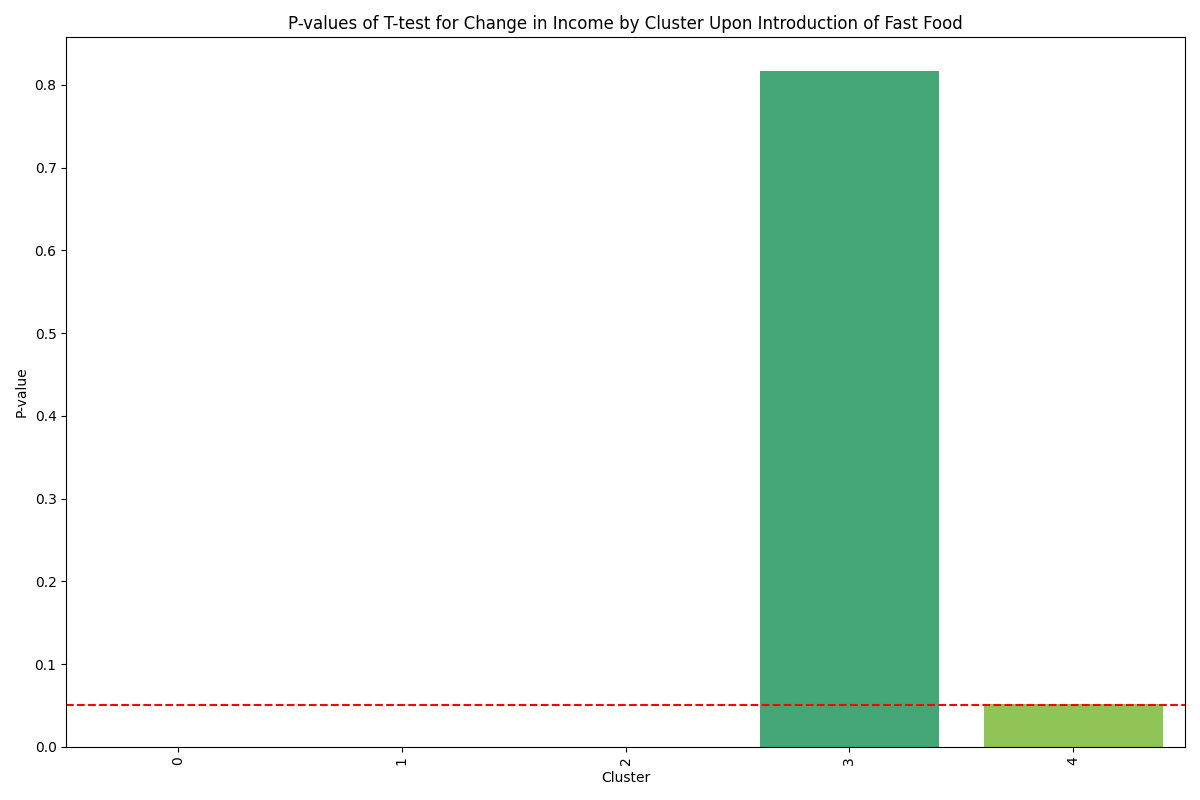
\includegraphics[scale=0.4]{propensity_matching_clusters_income.png}
    \caption{P-values of T-test for Change in Median Household Income by Cluster Upon Introduction of Fast Food}
    \label{fig:mental_health_pvalues}
\end{figure}

\paragraph{Cluster 0: Moderately Rural, Moderate Income}
\textbf{Cluster Characteristics:} This cluster consists of counties with a moderate rural population, middle-income levels, and moderate racial diversity. The analysis revealed that the introduction of fast-food restaurants in these counties was associated with a significant positive change in household income. The t-test results, with a strong positive t-statistic, suggest that in these counties, the economic benefits of fast food restaurant introduction might be linked to increased employment opportunities and local economic activity generated by these establishments.

\paragraph{Cluster 1: Highly Rural, Low Income}
\textbf{Cluster Characteristics:} This cluster is characterized by highly rural, economically disadvantaged counties with a high percentage of African American residents and elevated obesity rates. The analysis showed a significant negative impact on household income following the introduction of fast-food restaurants, as indicated by a negative t-statistic. This suggests that in these counties, the presence of fast-food restaurants may exacerbate economic challenges, possibly by diverting spending away from local businesses or by reinforcing unhealthy lifestyle choices that reduce overall economic productivity.

\paragraph{Cluster 2: Very Rural, Low to Moderate Income}
\textbf{Cluster Characteristics:} These counties are very rural, with low to moderate income levels and low racial diversity. The analysis indicated a moderate positive economic impact of fast food restaurant introduction, as reflected by the t-test results. The increase in household income may be attributed to the creation of low-wage jobs and the stimulation of local economic activity, although the effect was less pronounced than in Cluster 0.

\paragraph{Cluster 3: Urbanized, High Income, Diverse}
\textbf{Cluster Characteristics:} This cluster includes urbanized, affluent counties with significant ethnic diversity and lower obesity rates. The introduction of fast food restaurants had little to no measurable impact on household income in these counties, as evidenced by a near-zero t-statistic. This suggests that in wealthier, more economically stable areas, the introduction of fast-food restaurants does not significantly alter the economic landscape, likely due to the presence of diverse economic opportunities and robust local economies.

\paragraph{Cluster 4: Low Rural Population, High Income, Moderate Diversity}
\textbf{Cluster Characteristics:} Counties in this cluster have low rural populations, higher income levels, and moderate racial diversity. The analysis revealed a marginally significant positive impact on household income following the introduction of fast-food restaurants, as shown by the t-test results. This suggests that even in affluent areas, fast-food restaurants can contribute to economic growth, albeit to a lesser extent compared to more economically vulnerable regions.

\subsubsection{Cluster-Specific Insights and Policy Implications}
The results of the economic impact analysis highlight the nuanced effects of fast food restaurant introduction across different socioeconomic contexts:

\begin{itemize}
    \item \textbf{Cluster 0:} The significant positive economic impact observed in these moderately rural counties suggests that fast food restaurants can serve as important drivers of economic activity, particularly in regions where other economic opportunities may be limited.
    
    \item \textbf{Cluster 1:} The negative economic impact in these highly rural, low-income counties underscores the potential for fast-food restaurants to exacerbate existing economic challenges. Policymakers should consider these potential downsides when assessing the overall benefits of such establishments in economically disadvantaged areas.
    
    \item \textbf{Cluster 2:} The moderate positive impact in very rural counties with low to moderate income levels indicates that fast food restaurants can provide some economic benefits, although these are likely limited by the overall economic context of the region.
    
    \item \textbf{Cluster 3:} The negligible impact on household income in urbanized, affluent counties suggests that fast food restaurant introduction does not significantly alter the economic status quo in wealthier areas, where the economic ecosystem is more diverse and robust.
    
    \item \textbf{Cluster 4:} The marginally positive economic impact in affluent, moderately diverse counties highlights that even in wealthier areas, fast food restaurants can contribute to economic growth, though the effects are more subdued compared to regions with lower income levels.
\end{itemize}
\paragraph{Conclusion: Economic and Health Disparities in the Context of Fast Food Prevalence}

The model illustrates that the economic impact of fast-food restaurant introduction varies significantly across different socioeconomic and demographic contexts, mirroring the patterns observed in mental health outcomes. In highly rural, low-income counties with significant minority populations, such as those in Cluster 1, the economic consequences of fast food prevalence are largely negative, exacerbating existing challenges. These areas not only experience declines in household income, likely due to the diversion of spending away from local businesses, but also suffer from deteriorating mental health outcomes, as fast food establishments further entrench unhealthy lifestyle choices.

Conversely, in urbanized, affluent counties like those in Cluster 3, the introduction of fast-food restaurants has a negligible economic impact, reflecting a resilience also observed in mental health metrics. These wealthier areas benefit from diverse economic opportunities and robust healthcare systems that mitigate the negative effects of fast food prevalence. However, even in affluent areas such as Cluster 4, the model indicates that fast food can still contribute to economic and health declines, though to a lesser extent, suggesting that the adverse effects of fast food are not entirely contained by socioeconomic advantages.

Overall, the findings underscore that fast food restaurant introduction tends to reinforce existing economic and health inequalities, particularly in rural, low-income, and minority communities. This calls for targeted policy interventions that address both the economic and health vulnerabilities of these populations, while also recognizing that even affluent communities are not fully immune to the broader impacts of fast food proliferation.


\subsection{Investigating the Impact on Self-Reported Health Metrics of Fast Food Restaurant Introduction}

\subsubsection{Clustering and Data Overview}
The analysis of fair/poor health outcomes utilized the same clustering features as those used for the mental health and economic benefit analyses. However, obesity was excluded as a clustering feature in this analysis. This decision was made because obesity is closely related to the response variable (fair/poor health), and including it could have biased the clustering process. The objective was to focus on environmental effects on health outcomes without pre-grouping counties based on a feature highly correlated with the health metric being studied. The response variable was the proportion of people in the county who self-reported fair or poor health.

\noindent The figure below illustrates the p-values of the T-test conducted to assess the change in economic impact outcomes across different clusters following the introduction of fast food establishments, with significant results in all 5 out of the 5 counties.

% The figure environment for the image and its caption
\begin{figure}[h!]
    \centering
    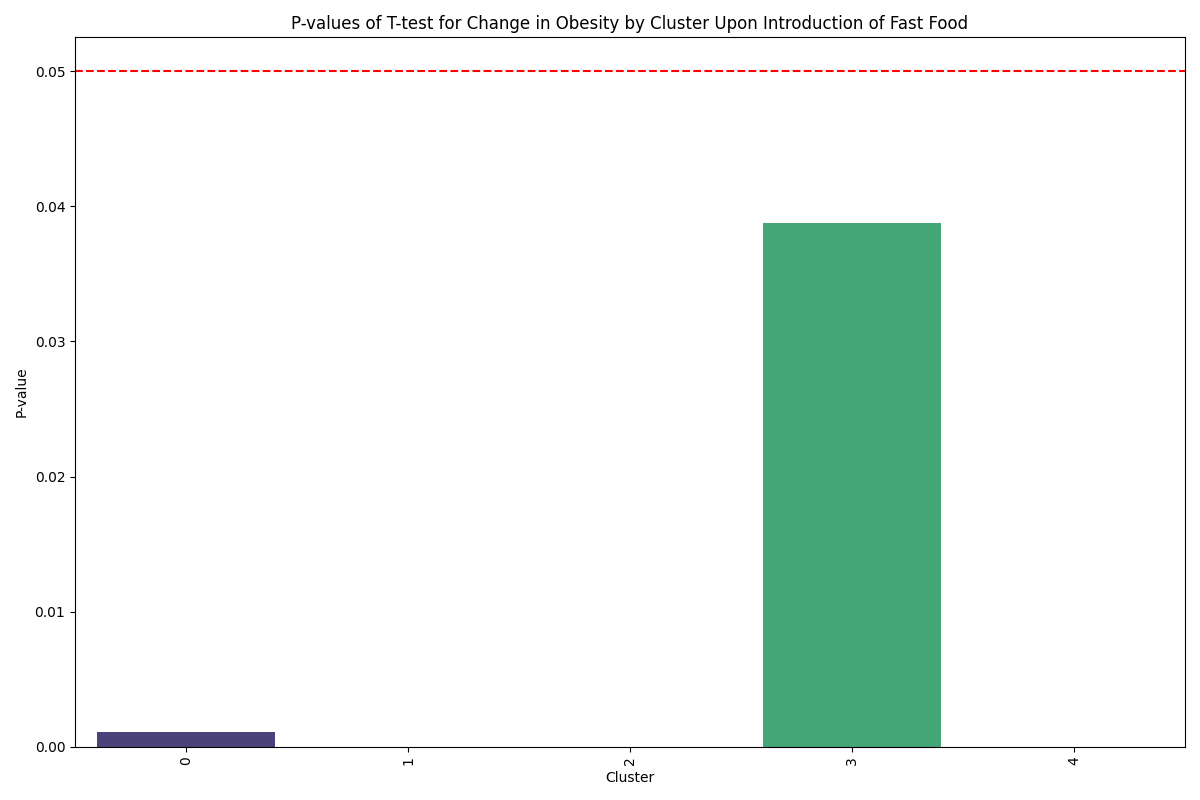
\includegraphics[scale=0.4]{propensity_matching_clusters_poorhealth.png}
    \caption{P-values of T-test for Change in Proportion of People Reporting Fair/Poor Health by Cluster Upon Introduction of Fast Food}
    \label{fig:mental_health_pvalues}
\end{figure}

\newpage
\subsubsection{Cluster-Specific Insights and Policy Implications}
\paragraph{Cluster 0: Moderately Rural, Predominantly Hispanic}
\textbf{Cluster Characteristics:} This cluster has a moderate rural population (~32.94\%), low household income (~\$42,551), and a predominantly Hispanic population (~47.04\%). The analysis showed a significant increase in the proportion of people reporting fair or poor health (t-statistic: 3.39, p-value: 1.08e-03), suggesting a decline in overall health following the intervention. The moderate rurality and low income, combined with the high Hispanic population, indicate that the introduction of fast-food restaurants may have negatively impacted the community’s health. This increase in fair/poor health could be related to increased fast food consumption or reduced access to healthcare and healthy food options.

\paragraph{Cluster 1: Moderately Rural, Moderate Income}
\textbf{Cluster Characteristics:} This cluster is characterized by a moderate rural population (~30.24\%), moderate household income (~\$53,815), and moderate racial diversity. The analysis revealed a substantial increase in the proportion of people reporting fair or poor health (t-statistic: 20.25, p-value: 3.18e-75), indicating a significant decline in overall health status. Despite the moderate income levels, the introduction of fast-food restaurants appears to have had a strongly negative impact on health, possibly due to lifestyle changes, increased stress, or reduced physical activity.

\paragraph{Cluster 2: Highly Rural, Low Income}
\textbf{Cluster Characteristics:} This cluster includes counties with a very high rural population (~78.10\%), low household income (~\$40,762), and low racial diversity. Unlike the other clusters, Cluster 2 saw a significant decrease in the proportion of people reporting fair or poor health (t-statistic: -12.40, p-value: 2.33e-32), indicating an improvement in overall health status. This positive outcome might be due to increased health awareness, community support, or effective local health initiatives in these highly rural areas.

\paragraph{Cluster 3: Urban, High-Income, Diverse}
\textbf{Cluster Characteristics:} This cluster consists of urbanized, high-income counties with significant racial diversity. The introduction of fast food restaurants led to a modest but significant decrease in the proportion of people reporting fair or poor health (t-statistic: -2.14, p-value: 3.87e-02), indicating a slight improvement in health. The high household income and urban setting likely provided better access to healthcare and healthier lifestyle options, contributing to this positive health outcome.

\paragraph{Cluster 4: Highly Rural, Low-Income, Predominantly African American}
\textbf{Cluster Characteristics:} Cluster 4 is characterized by a high rural population (~59.27\%), the lowest household income among all clusters (~\$35,758), and a predominantly African American population (~40.73\%). The analysis revealed a significant increase in the proportion of people reporting fair or poor health (t-statistic: 8.24, p-value: 1.12e-14), suggesting a decline in health status. The combination of high rurality, low income, and limited access to healthcare likely made this community particularly vulnerable to negative health impacts from the introduction of fast food restaurants.

\subsubsection{Qualitative Conclusions Based on P-Values and Cluster Composition}
The analysis of p-values and t-statistics across clusters provides key insights:

\begin{itemize}
    \item \textbf{Cluster 0:} The significant increase in fair/poor health outcomes suggests that fast food restaurant introduction has a substantial negative impact on health in moderately rural, predominantly Hispanic counties.
    \item \textbf{Cluster 1:} The strong negative impact observed in this moderately rural, moderate-income cluster highlights the potential health risks associated with increased fast food availability, even in economically stable areas.
    \item \textbf{Cluster 2:} The improvement in health outcomes in highly rural, low-income counties suggests that these communities may benefit from health interventions or community support, despite low income and rural isolation.
    \item \textbf{Cluster 3:} The slight improvement in health in urban, high-income counties indicates that higher income and access to resources may mitigate the negative effects of fast food availability.
    \item \textbf{Cluster 4:} The significant decline in health outcomes in highly rural, low-income, predominantly African American counties underscores the need for targeted health interventions in vulnerable communities facing multiple socioeconomic challenges.
\end{itemize}

\paragraph{Conclusion: Health Disparities and Environmental Influences in Fast Food Prevalence}

The model underscores that the introduction of fast-food restaurants has a significant and varied impact on self-reported health outcomes across different clusters, reflecting broader patterns of inequality similar to those observed in both mental health and economic analyses. In predominantly Hispanic, moderately rural counties (Cluster 0) and low-income, predominantly African American counties (Cluster 4), the prevalence of fast food is linked to a marked increase in the proportion of people reporting fair or poor health. This is consistent with findings from other research that fast food availability exacerbates existing health disparities, particularly in communities already burdened by limited access to healthcare and healthy food options.

In contrast, urbanized, affluent counties (Cluster 3) show a slight improvement in self-reported health outcomes, likely due to better access to healthcare and healthier lifestyle choices, paralleling the resilience seen in mental health and economic outcomes. However, even in these more resilient clusters, the pervasive influence of fast food still presents challenges, albeit to a lesser extent.

Interestingly, the model also reveals a unique trend in highly rural, low-income counties (Cluster 2), where self-reported health outcomes improved despite increased fast food availability. This suggests that other factors, such as community-driven health initiatives or increased awareness, may play a critical role in mitigating the negative effects of fast food in these isolated regions. This might also be because the introduction of fast food into the community revives the economy and provides more opportunities.

Overall, these findings highlight the need for targeted public health interventions that address the specific vulnerabilities of rural, low-income, and minority communities. While urban areas may demonstrate resilience, the broader public health implications of fast food prevalence demand attention across all socioeconomic contexts to reduce health disparities and promote equity.


\subsection{Analysis of Healthy Fast Food}

According to a recent report by investors, stocks of healthy fast-food companies are rising. \cite {investors2024_chipotle} Despite their higher prices, as reported in The Wall Street Journal \cite{wsj2024_chipotle}, consumer demand for these healthier options remains strong. 

In this analysis, we use Chipotle Mexican Grill as a representative of the group that values healthier and more sustainable food options, while McDonald's serves as a representative of traditional fast food known for its widespread availability, affordability, and appeal to a broad demographic. Figure 8 represents the annual employee count across three major fast-food restaurants from 2009 to 2023, utilizing historic data from \cite{mcdonalds2024_employees} and \cite{macrotrends2024_chipotle_employees}. 

In figure 8, one can observe a striking trend: Chipotle's employee count has grown consistently and substantially over this period, reaching levels comparable to McDonald's by 2023. This growth trajectory challenges the conventional wisdom that only traditional fast food can be a significant job creator in the food service industry. Despite its higher prices and focus on healthier options, Chipotle's expansion demonstrates that health-oriented fast food chains can contribute significantly to employment and economic growth. The data suggests that the shift towards healthier fast food options does not necessarily come at the expense of job creation or economic impact. In fact, it indicates that promoting and expanding healthier fast food concepts could have positive effects on both employment and public health outcomes, potentially offering a win-win scenario for economic and health policy considerations. \cite{chipotle2024_locations}

\begin{figure}[h!]
    \centering
    \includegraphics[width=\linewidth]{images/image2.jpg}
    \caption{Annual Employee Count across Fast Food Restaurants}
    \label{fig:employees}
\end{figure}

To understand the impact fast food has on different demographic and racial groups across various locations, we analyze the distribution of McDonald's and Chipotle locations across states. Figure 9 compares this distribution. \cite{csun2024_mcd}

The data reveals that Chipotle, representing healthier fast food options, has a significant presence across diverse states, not just in metropolitan areas. Key points include:

\begin{itemize}
    \item Chipotle has locations in nearly all states represented, indicating a national presence.
    \item The ratio of McDonald's to Chipotle locations varies by state, potentially reflecting local preferences and economic conditions.
    \item Chipotle's presence in states with large rural populations challenges the assumption that healthier fast food is exclusively urban.
\end{itemize}

\begin{figure}[h!]
    \centering
    \includegraphics[width=\linewidth]{images/image3.jpg}
    \caption{Number of McDonald's and Chipotle Locations per State}
    \label{fig:employees}
\end{figure}

Figure 10 compares ESG scores of Chipotle and McDonald's, based on Market Beat data \cite{marketbeat2024} \cite{marketbeat2024_cmg}. Key findings:

Health Metrics:
\begin{itemize}
    \item Chipotle outperforms McDonald's across all categories.
    \item Both show negative scores for Overall Health, Physical and Mental Diseases.
\end{itemize}

Environment Metrics:
\begin {itemize}
    \item Chipotle leads in Overall Environment and GHG Emissions.
    \item McDonald's performs slightly better in Non-GHG Emissions and Waste.
\end {itemize}

This data suggests Chipotle maintains higher ESG standards, particularly in health-related metrics, while McDonald's shows competitive performance in some environmental categories.

\begin{figure}[h!]
    \centering
    \includegraphics[width=\linewidth]{images/image4.jpg}
    \caption{ESG Scores of Major Fast-Food Chains}
    \label{fig:employees}
\end{figure}


\newpage

\section{Conclusion}

The cycle perpetuated by the financial interests of processed food corporations has far-reaching implications for public health and socioeconomic stability. Our analysis highlights how the strategic interests of these corporations contribute to a cycle of poor mental health, low income, adverse employment conditions, and deteriorating physical health. The prevalence of fast food and ultra-processed foods is intricately linked to corporate profitability, but this comes at the cost of public well-being.

The analysis conducted in this report highlights the profound and varied impacts of fast food prevalence on public health and economic outcomes across different communities in the United States. Our findings reveal that the introduction of fast-food establishments exacerbates existing health and economic disparities, particularly in rural, low-income, and minority communities. These areas, already burdened by limited access to healthy food and healthcare, are further disadvantaged by the proliferation of fast food, which leads to worsening mental and physical health outcomes and diminished economic stability.

Conversely, urbanized, affluent counties demonstrate resilience to the negative effects of fast food, benefiting from diverse economic opportunities and robust healthcare systems. However, even these areas are not entirely immune to the broader public health implications of fast food proliferation, suggesting that the adverse effects of processed food are pervasive and not easily contained by socioeconomic advantages.

The rise of healthier fast food alternatives, as exemplified by the growth of chains like Chipotle, offers a potential avenue for mitigating some of the negative impacts associated with traditional fast food. However, the success of these healthier options in promoting both economic growth and public health underscores the need for a systemic shift in how food environments are structured and regulated.

In conclusion, targeted public health interventions are essential to address the specific vulnerabilities of rural, low-income, and minority communities.

These should include:
\begin{itemize}
    \item \textbf{Regulation of Marketing Practices:} Stricter regulations on how processed foods are marketed, particularly to vulnerable populations such as children and low-income communities.
    \item \textbf{Promotion of Healthier Alternatives:} Incentives for businesses to offer and promote healthier food options, along with public education campaigns to raise awareness about the benefits of nutritious diets.
    \item \textbf{Economic Support for Affected Communities:} Investment in economic development programs that provide alternative employment opportunities and support local businesses, reducing reliance on low-wage jobs in the fast food industry.
    \item \textbf{Healthcare Access and Education:} Enhanced access to healthcare services and nutrition education, particularly in areas with high rates of processed food consumption and related health issues.
\end{itemize}

Policies aimed at reducing the prevalence of fast food and promoting healthier alternatives could help break the cycle of poor health and economic disadvantage that currently traps many communities. By fostering a food environment that supports well-being and equity, we can take significant strides toward building a healthier future for all.

Future research should continue to explore the complex relationships between dietary habits, health outcomes, and socioeconomic factors. By understanding these dynamics, policymakers can develop more effective strategies to promote public health and economic equity, ultimately disrupting the cycle perpetuated by corporate interests in the processed food industry.


\newpage

\section{Appendices}

\begin{figure}[h!]
    \centering
    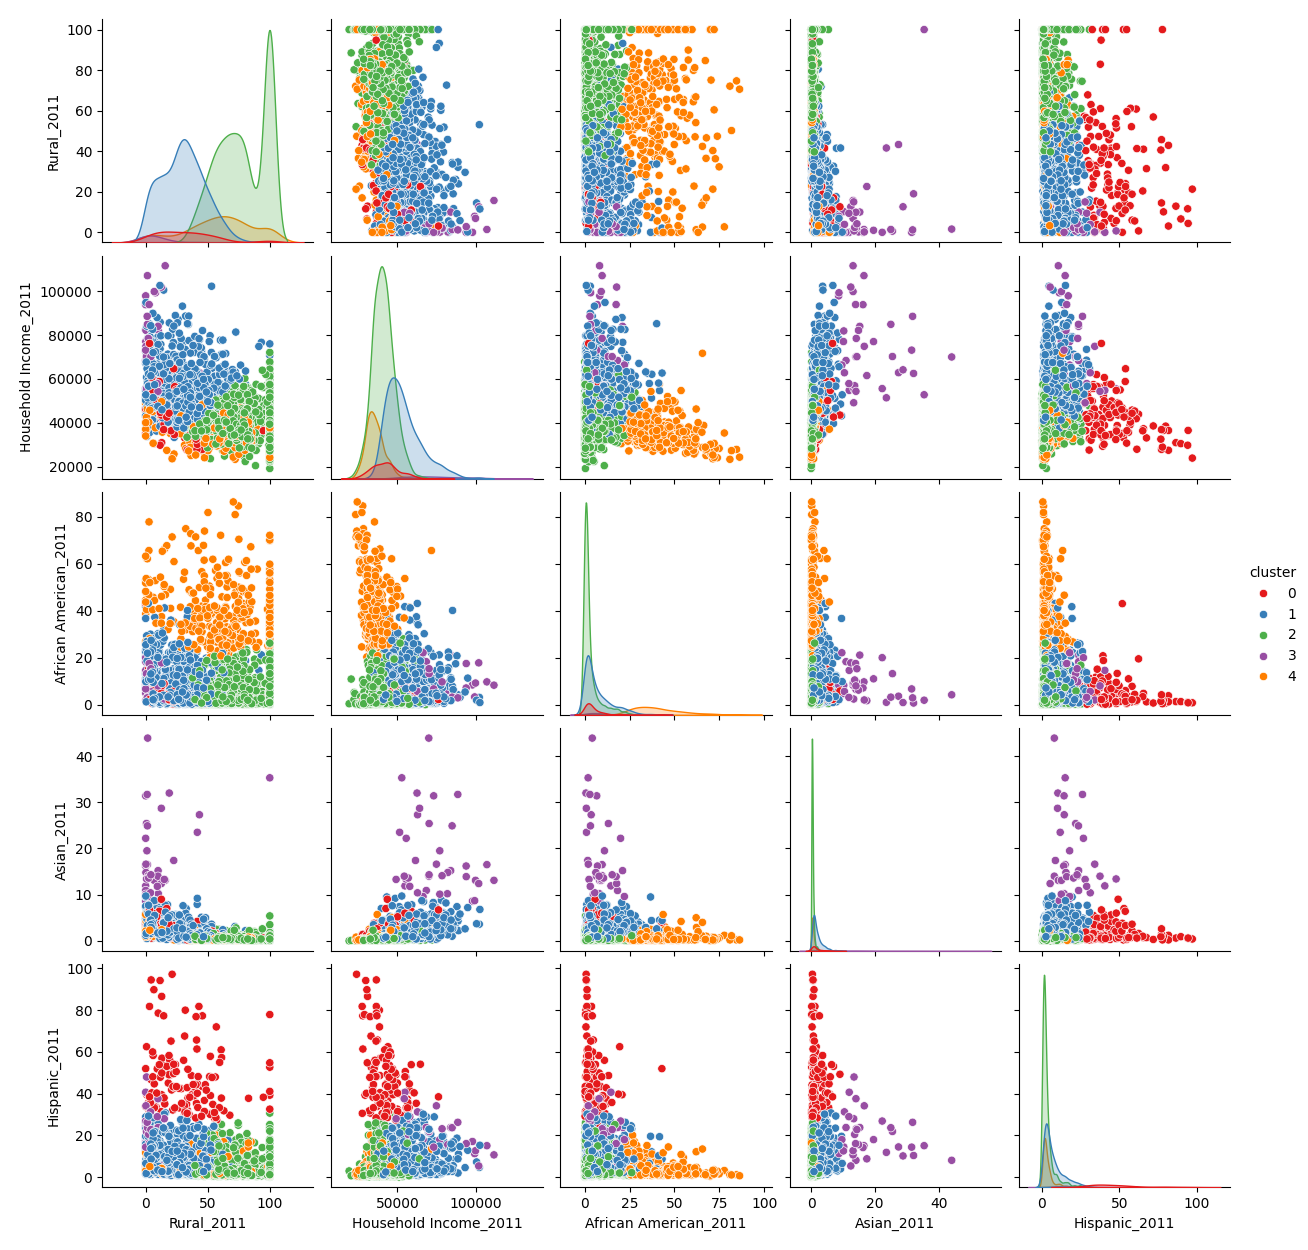
\includegraphics[width=\linewidth]{Clustering of counties.png}
    \caption{Pair wise features plot for clusters of counties used for propensity score matching}
    \label{fig:clustering}
\end{figure}

\newpage
\printbibliography[heading=bibintoc]
\addcontentsline{toc}{section}{References}

\end{document}

